% Beamer slide template prepared by Tom Clark <tom.clark@op.ac.nz>
% Otago Polytechnic
% Dec 2012

\documentclass[10pt]{beamer}
\usetheme{Dunedin}
\usepackage{graphicx}
\usepackage{fancyvrb}
\usepackage{hyperref}

\newcommand\codeHighlight[1]{\textcolor[rgb]{1,0,0}{\textbf{#1}}}

\title{Kubernetes}

\author[I720]{Virtualisation}
\institute[Otago Polytechnic]{
  Otago Polytechnic \\
  Dunedin, New Zealand \\
}
\date{}
\begin{document}

%----------- titlepage ----------------------------------------------%
\begin{frame}[plain]
  \titlepage
\end{frame}


\begin{frame}
  \frametitle{Ok, what is it?}
   
   \begin{itemize}
     \item Kubernetes is a container orchestration system.
     \item More full featured than Compose/Swarm, and hence more complicated.
     \item Works with Docker and other container systems.
     \item Originally developed at Google, since spun off and currently managed by the Cloud Native Computing Foundation.
     \item \url{https://kubernetes.io}
   \end{itemize}
\end{frame}
 
  
\begin{frame}
 \frametitle{Architecture}
  
   \begin{center}
     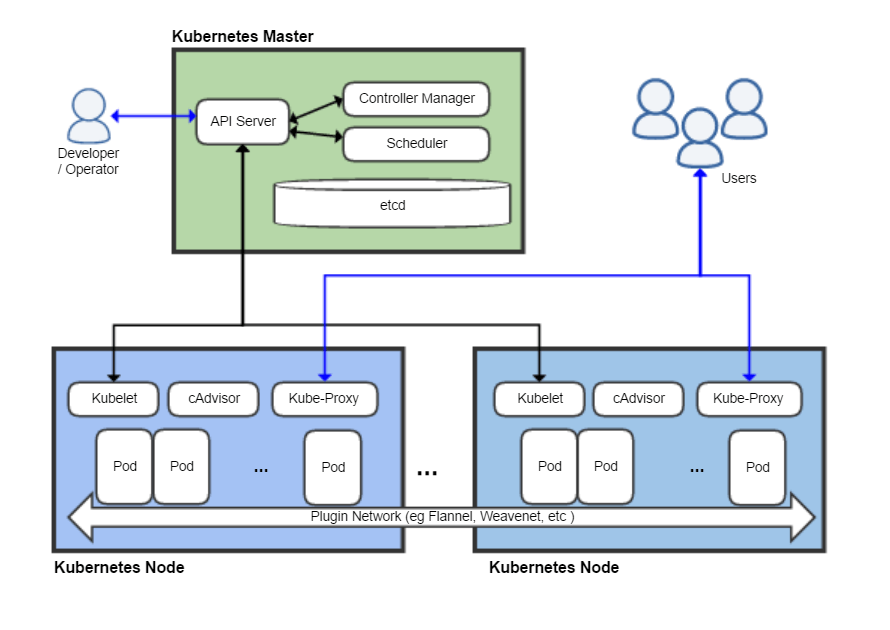
\includegraphics[scale=0.3]{arch}\footnote{Image from Wikipedia}
     \end{center}
\end{frame}

\begin{frame}
  \frametitle{Clusters}
   
   A Kubernetes cluster is consists of multiple servers (physical or virtual), organised as 
   \begin{itemize}
     \item One or more masters that coordinates the orchestration
     \item One or more nodes
        \end{itemize}
\end{frame}

\begin{frame}
  \frametitle{Pods}
   
   The fundamental unit of Kubernetes is the Pod.
   \begin{itemize}
        \item Pods consist of one or more containers and related resources.
        \item Elements of a pod are all deployed on the same node.
        \item We can deploy multiple instances of the same kind of pod.
        \item All the elements of a pod share the same internal IP address.
        \item The configuration to run a set of Pods is called a Deployment.
        \end{itemize}
\end{frame}

\begin{frame}
  \frametitle{Services}
   
   Pods can be organised to provide a Service
   \begin{itemize}
       \item The pods that comprise a service can be of different types.
       \item Service are exposed internally within a cluster.
       \item Services can also be exposed to users outside the cluster over the larger network.
     \end{itemize}
\end{frame}


\begin{frame}
  \frametitle{Lab}
   Do the ``Kubernetes Basics'' tutorial at \url{https://kubernetes.io/docs/tutorials/kubernetes-basics/}
   
\end{frame}

\end{document}
